\section{Investigation into effects of disruptive events.}
\label{sect:exp_disruption}

.During an observing night a variety of disruptive events can take place. 
\begin{itemize}
\item Bad weather can stop observing for either an extended period or, when the weather variables are close to the upper and lower limits, for a series of short intervals, refered to as \emph{spikes}.
\item Mechanical, electrical and software problems can cause pauses in observing while recovery systems take over to effect repairs.
\end{itemize}

The lengths and frequencies of these interruptions are variable and have already been characterized (Sect.~\ref{sect:character}). In the case of a dispatch scheduler we might expect that little effect would be seen. Such schedulers are myopic, a feature generally regarded as non-optimal, though as we have already seen this can sometimes be advantageous. For the look-ahead schedulers which are investing effort to obtain the best overall reward by allocating appropriately to each time-slot, we might expect some potential degradation in performance.

A series of simulations were performed in order to investigate the effects of such disruptive events on scheduling performance.

\subsection{Methodology}
Simulations were performed using BDS and QLAS with horizons of length 0.5, 1, 2, 3, 4 and 6 hours. The environment model was set to fixed with good seeing. The Phase 2 model was populated with groups with small execution windows spread through the night. This means that the size of the pool remains more or less constant through the night but individual groups if missed are unlikely to be rescheduled later. The distribution of scores was arranged so that most groups are roughly level while a small fraction have distinctly larger scores. This is an attempt to \emph{help} the QLAS to achieve higher scores than BDS as these are the sort of conditions where it might be expected to perform better and has in a sense \emph{more to lose}.

In anticipation that the frequency of disruption rather than the total length of disruption is likely to have more effect, the simulations were performed with different numbers of disruptions but with the same total length (1 hour) of disruption time. A number $N$ of disruptions each of the same length were scheduled to occur at random times during the night. We expect the total reward for an observing night to be reduced if a fraction of the night $\epsilon$ is \emph{offline}. Consequently the summed reward for the \emph{no-disruption} case ($N = 0$) is down-scaled by the factor $1-\epsilon$. A total of 1000 simulations were performed for each combination of scheduler and number of disruptions over a single night of length 12 hours.

\subsection{Results}
The results of the simulations are shown in Fig.~\ref{fig:disrupt} with derived statistics in Table.~\ref{b:f111}. For clarity, the line shown for BDS is an average of the results taken using the full range of \emph{number of disruptive events}. The BDS results were fairly constant around the baseline value of $\sim 118$ with around $\pm 3.5$\% variation. For QLAS the situation is somewhat different. As can be seen, the effect of increasing numbers of short disruptions is to reduce the total reward. This effect is more noticeable for the longer horizon schedulers. At $n_e=12$ QLAS with H=2 suffers a drop of 8.4\% $\pm 5.6$\% whilst at $n_e=0$ it performs better than BDS by 8.6\% $\pm 4.3$. We might infer that in these cases, because such a large investment has been made in obtaining the optimum sequence, any disruptions lead to higher instantaneous loss. We should however take note of the size of the error bars. These indicate the background level of variation between individual scheduling runs due to variations in execution time and ODB content. Overall the effect of disruption is quite small.

\begin{figure}[h]
\begin{center}
 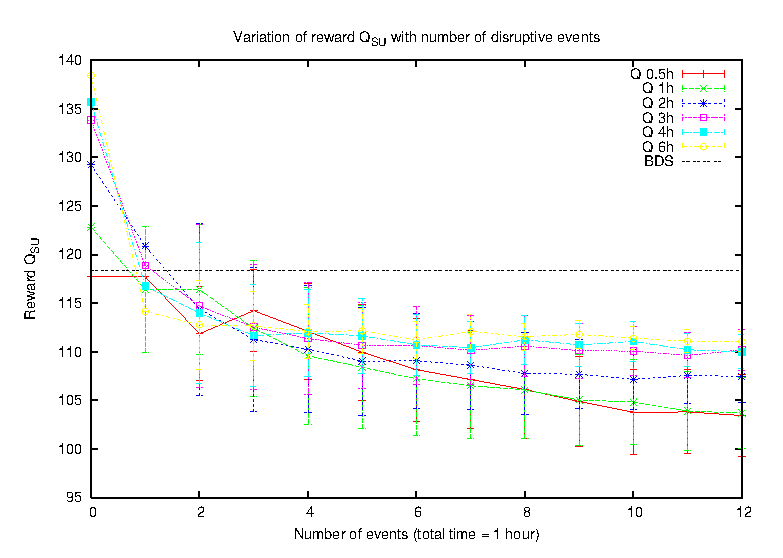
\includegraphics[scale=1.0, angle=0]{figures/disruption.eps}
 \caption[Effect of variation of number of disruptive events $N$ on total schedule reward $Q_{SU}$.] 
   {Effect of variation of number of disruptive events on schedule reward $Q_{SU}$. Results for $N = 0$ are scaled by a factor $1/(1-\epsilon)$ where $\epsilon$ is the fraction of night distrupted.}
\label{fig:disrupt}
\end{center}
\end{figure}

\subsection{Summary and conclusions}
Disruptive events, breaks in the natural execution cycle due to weather, mechanical or computer problems were investigated to determine their effect on schedule quality. It was found that for a given total disruption time, a large number of small disruption had a worse effect than a few long events. The effect was seen to be more pronounced for longer look-ahead horizons. The despatch schedulers were unnaffected, the \emph{myopic advantage}.
